\documentclass[11pt,handout]{beamer}

\usepackage{tcolorbox}
\usepackage{minted}
\usepackage{pdfpages}
\usepackage{sourcecodepro}
\usepackage{graphicx}
\usepackage{amsmath}
\usepackage{bussproofs}
\usepackage{mathpartir}
\usepackage{prooftrees}
\usepackage{color}
\usepackage{algorithmicx}
\usepackage{algpseudocode}

\usetikzlibrary{calc}

\graphicspath{{img/}}

\usetheme{CambridgeUS}

\title[FDS Seminar]{Foundations of Dependable Systems Seminar : \\ 
  Bisimulation and Model Checking}
\author{Noé Zufferey, Sylvain Julmy}
\date{\today}

\begin{document}

\maketitle

%%%%%%%%%%%%%%%%%%%

\begin{frame}
 \frametitle{Model Checking 1}
 The paper focus on the checking of invariance properties.
 A logical proposition is either true or false for each state.
 Can the analysed state system reach a system that does not correspond to this logical proposition ?
\end{frame}

\begin{frame}
 \frametitle{Model Checking 2} 
 A model checker has to analyse the entire transition state spaces.
 Some methods are used to reduce the size of the state space.
 One of them is bisimilution minimization.
 
 The paper study a model checking method which uses bisimilution minimization.
 Minimized sytems are faster to check.
\end{frame}

\begin{frame}
 \frametitle{Model Checking 3} 
 A formal model for symbolic model checking can be : \\ \vspace{10pt}
 
 $ \langle S, R, AP, L, init \rangle$
 \begin{itemize}
  \item $S$ : set of states
  \item $R$ : the transitions over $S$
  \item $AP$ : a set of atomic prposition
  \item $L$ : $S \times AP$, set of pairs atomic prppositions and the states they are true with.
  \item $init$ : the initial state
 \end{itemize}

\end{frame}

\begin{frame}
 \frametitle{Bisimilution minimization}
 The purpose is to reduce the number of states.
 Bisimulation minimization algorithms analyse a transition state space to find set of states
 that are equivalent with a given logical proposition.
 
 Both state systems, the first one and the minimization are bisimilar in respect with a logical proposition.
 They can simulate each other for the model checking.
\end{frame}

\begin{frame}
 \frametitle{Bisimilution minimization 2}
 A common way to Minimize state systems is to split the state space in classes in which states have
 the main behaviour regarding the logical prposition.
 
 Then each class is repeatidly split into new classes until all states of a class agree on the type of their successor.
\end{frame}

\begin{frame}
 \frametitle{Bisimilution minimization 3}
 A naïve way to compute a bisimultation minimization is to repeatidly look for states that are not bisimilar and/or their succesor are not bisimilar.\\\\
 \vspace{10pt}
 \begin{align*}
   & \exists ap \in AP \lnot (L(s_1, ap) \Leftrightarrow L(s_2, ap)) \lor \\
   & \exists s'_1 R(s_1, s'_1) \land \lnot (\exists s'_2 (R(s_2, s'_2) \land B(s'_1, s'_2))) \lor \\
   & \exists s'_2 R(s_2, s'_2) \land \lnot (\exists s'_1 (R(s_1, s'_1) \land B(s'_1, s'_2)))
 \end{align*}
\end{frame}

\begin{frame}
 \frametitle{Bisimilution minimization 4}
 The first line : \vspace{10pt}
 
  $\exists ap \in AP \lnot (L(s_1, ap) \Leftrightarrow L(s_2, ap))$ \vspace{10pt}
  
  looks for states that are not directly bisimilar in respect with the logical prposition.
  
  The two last lines : \vspace{10pt}
  
  $\exists s'_1 R(s_1, s'_1) \land \lnot (\exists s'_2 (R(s_2, s'_2) \land B(s'_1, s'_2))) \lor
  
  \exists s'_2 R(s_2, s'_2) \land \lnot (\exists s'_1 (R(s_1, s'_1) \land B(s'_1, s'_2)))$ \vspace{10pt}
  
  look for states whose successors are not bisimilar.
\end{frame}

\begin{frame}
 \frametitle{Bisimilution minimization 5}
 The naïve algorithm takes into account the unreachable states.
\end{frame}

\begin{frame}
 \frametitle{Terminology}
 The paper difines a number of terms that are usefull when speaking of bisimulation minimization algorithms.
\end{frame}

\begin{frame}
 \frametitle{Terminology 2}
 \begin{itemize}
  \item block : set of states
  \item block's representative : the state that represent its whole blocks
  \item partition : set of blocks
  \item initial partition : partition of the two block (good and bad) that are used at the beggining of the algorithms
  \item good block : initial block composed by states that satisfy the given invariant property
  \item bad block : initial block composed by states that do not satisfy the given invariant property
 \end{itemize}
\end{frame}

\begin{frame}
 \frametitle{Terminology 3}
 \begin{itemize}
  \item refine : a partition $P_1$ refines a partition $P_2$ iff each blck of $P_1$ is contained in blocks of $P_2$
  \item reachable : a state is reachable if their is an existing path between de initial state and this state. A block is reachable if containing a reachable state.
  \item stable : a block $B_1$ is stable with a block $B_2$ iff every state in $B_1$ have transition with at least one state of $B_2$ or if no state in $B_1$ have transition with states in $B_2$
  \item splitter : a splitter of a block is a block that the first black is not stable with
 \end{itemize}
\end{frame}

\begin{frame}
 \frametitle{Invariance checking}
 The paper studies invariance checking. An invariance property is true iff every reachable state satisfies it.
 Invariance checking can be executed in two ways
 \begin{itemize}
  \item forward reachability
  \item backward reachability
 \end{itemize}
 Backward reachability (BR) is closely related to bisimilution minimization. 
\end{frame}

\begin{frame}
 \frametitle{Backward reachability}
 BR has two set of states. The frontier states $F$ that represent the new discovered states and the explored states $S$.
 BR iterates the following equations : \vspace{10pt}
 
 $F_0 = Bad
 
 F_{i + 1} = pre(F_i) - S_i$ \vspace{10pt}
 
 $S_0 = Bad
 
 S_{i + 1} = pre(F_i) \cup S_i$ \vspace{10pt}
 
 The iteration stop either if $F_i = \emptyset$ or if $init \in F_i$.
\end{frame}

\begin{frame}
 \frametitle{Backward reachability 2}
 The lower bound for BR is $n \cdot (M + U + D + 2E + I)$, with $n$ the number of iteration to terminate.
 
 $n$ is the length of th shortest path between the initial state and a bad state or $n$ is the length of the longest acyclic state from a good state to a bad state.
\end{frame}

\begin{frame}
 \frametitle{Algorithms}
 The paper study 3 diferent algorithms that apply bisimulation minimization for symbolic model checking : \vspace{10pt}
 
 \begin{itemize}
  \item PT
  \item BFH
  \item LY
 \end{itemize} \vspace{10pt}
 
 Each algorithm has been modified for model checking purpose. The authors added termination condition since the invariance has been proven true or false.
 \end{frame}

\begin{frame}
 \frametitle{PT algorithm}
 PT stands for Paige-Tarjan.
 
 PT stabilizes every block (reachable and unreachable). It selects splitters to stabize the system instead of block to split.

 Two partition are used in PT. The current partition $Q$ and the previous partition $X$. $Q$ refines $X$. That basically means that $Q$ contains more blocks.
 
 The algorithm repeatidly look for blocks of $X$ that contains states from multiple blocks of $Q$. This kind of blocks is called of compound block.
 Then, the compound block is splitted.
 
 A Block is marked if it contains a bad state. The algorithm fail if init is marked.
\end{frame}

\begin{frame}
 \frametitle{PT algorithm 2}
  The marking had been added to support early termination. If a splitter B is marked, every block that reach B is marked.
  So, this PT algorithm contains at most 1 marked block (and if zero, it stop with violation)
  
  Furthermore, the algorithm never split a marked block, split a marked block is not helpful
\end{frame}

\begin{frame}
 \frametitle{PT algorithm 3}
  \begin{itemize}
   \item Select a refining block.
   \item Update X
   \item Split the block containing elements that are predecessors of the splitter
  \end{itemize}
\end{frame}

\begin{frame}
 \frametitle{PT algorithm 4}
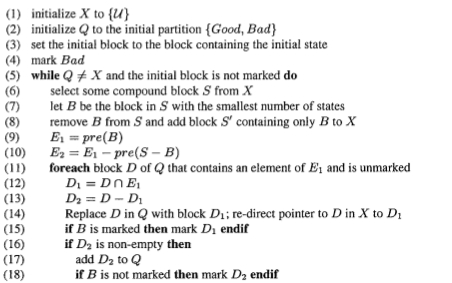
\includegraphics{figures/algo_part1}
\end{frame}

\begin{frame}
 \frametitle{PT algorithm 5}
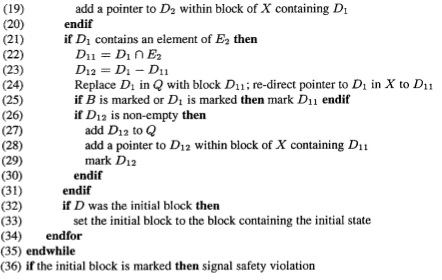
\includegraphics{figures/algo_part2}
\end{frame}

\begin{frame}
 \frametitle{PT algorithm 5}
The lower bound for PT is $n \cdot (2M + D + I + E)$, with n the number of while iterations
\end{frame}

%%%%%%%%%%%%%%%%%%%%%

\begin{frame}
  \frametitle{LY}
  The Lee-Yannakakis algorithm
\end{frame}

\begin{frame}
  \frametitle{LY - idea}
  \begin{itemize}
  \item Stabilize only reachable blocks.
  \item Reachable block use a representative that has to be reachable.
  \item The first state is the representative for the initial block.
  \item To find new reachable state, we look for transition from representative
    of reachable state to state from unreachable block.
  \end{itemize}
\end{frame}

\begin{frame}
  \frametitle{LY - idea}
  Two loops :
  \begin{itemize}
  \item Search new, reachable blocks
  \item Stabilize reachable but unstable blocks
  \end{itemize}
\end{frame}

\begin{frame}
  \frametitle{LY - termination}
  With the exception of the initial block, all new blocks created by the
  algorithm have paths to the bad block.
\end{frame}

\begin{frame}
  \frametitle{LY - termination}
  Therefore, when a second block becomes reachable, the algorithm should raise a
  violation and terminate.
\end{frame}

\begin{frame}
  \frametitle{LY - new algorithm}
  Basic idea\footnote{Very similar to BR} :
  \begin{itemize}
  \item Search new reachable blocks.
  \item Stabilize reachable but unstable blocks.
  \item When a second block becomes reachable $\to$ raise a violation.
  \end{itemize}
\end{frame}

\begin{frame}
  \frametitle{LY - search}
  To search for new reachable block, the algorithm is searching from all the
  successors of the initial state if one of those is in a different block.

  \pause
  \vspace*{1cm}

  The algorithm also determine if the initial block has to be stabilized or not.
\end{frame}

\begin{frame}[fragile]
  \frametitle{LY - search}
  \begin{algorithmic}
    \State{$D := post(B)$}
    \ForAll{$\langle {C,q} \rangle \in post(init)$}
    \If{$B \neq C$}
    \State{raise violation}
    \EndIf
    \If{$B \cap pre(C) \neq B$} \Comment{Not all predecessors of $B$ are in $B$}
    \State{$B$ is not stable}
    \EndIf
    \State{$D := D - C$}
    \EndFor
    \If{$D \neq \emptyset$} \Comment{$post(init) = \emptyset$}
    \State{$B$ is not stable}
    \EndIf
  \end{algorithmic}
\end{frame}

\begin{frame}[fragile]
  \frametitle{LY - search}
  \begin{columns}
    \begin{column}{0.5\textwidth}
      \begin{align*}
        & queue := \emptyset \\
        & partition = \{B, Bad\} \\
        & init = G_0 \\
        & B = \{G_0,\dots,G_2\}\\
        & Bad = \{B_0,B_1\} \\
        & block_{init} = \langle B,init \rangle \\
        & D = post(B) = \{ B,Bad \}
      \end{align*}
    \end{column}
    \begin{column}{0.5\textwidth}%
      \newcommand*{\con}[2]{(#1) edge [bend left] node {} (#2)}
\begin{tikzpicture}[->,shorten >=1pt,auto,node distance=1.3cm,
                thick,main node/.style={circle,draw,font=\bfseries}]
	\node[main node] (0) {$G_{0}$};
	\node[main node] (1) [below of = 0] {$G_1$};
	\node[main node] (2) [below of = 1] {$G_2$};
	
	\node[main node] (B0) [right of = 0] {$B_{0}$};
	\node[main node] (B1) [below of = B0] {$B_{1}$};
	\path
	\con{0}{1} \con{1}{0}
	\con{1}{2} \con{2}{1}
	\con{B0}{B1}
	(2) edge [bend left] (B1)
;
\end{tikzpicture}
    \end{column}
  \end{columns}
\end{frame}
  
\begin{frame}[fragile]
  \frametitle{LY - search}
  \begin{columns}
    \begin{column}{0.5\textwidth}
      \begin{align*}
        & post(init) = \{B\} \\
        & \langle {C,q} \rangle = \langle {B,init} \rangle \\
        & pre(C) = \{ B \} \\
        & \{B\} \cap pre(C) = \{B\} == \{B\} \\
        & D = \{B,Bad\} - \{B\} = Bad \\
        & D \neq \emptyset \to enqueue(\langle {B,init} \rangle)
      \end{align*}
    \end{column}
    \begin{column}{0.5\textwidth}%
      \newcommand*{\con}[2]{(#1) edge [bend left] node {} (#2)}
\begin{tikzpicture}[->,shorten >=1pt,auto,node distance=1.3cm,
                thick,main node/.style={circle,draw,font=\bfseries}]
	\node[main node] (0) {$G_{0}$};
	\node[main node] (1) [below of = 0] {$G_1$};
	\node[main node] (2) [below of = 1] {$G_2$};
	
	\node[main node] (B0) [right of = 0] {$B_{0}$};
	\node[main node] (B1) [below of = B0] {$B_{1}$};
	\path
	\con{0}{1} \con{1}{0}
	\con{1}{2} \con{2}{1}
	\con{B0}{B1}
	(2) edge [bend left] (B1)
;
\end{tikzpicture}
    \end{column}
  \end{columns}
\end{frame}

\begin{frame}[fragile]
  \frametitle{LY - stabilization}
  \begin{algorithmic}[1]
    \While{$B$ is not stable}
    \State{Mark $B$ as stable}
    \State{Compute the frontier of $B$}
    \State{Let $B'$ the state of $B$ that can only reach $B$}
    \State{Let $B''$ the state of $B$ that can reach a bad block}
    \If{$\emptyset \neq B' \cap pre(B') \neq B'$ or $\emptyset \neq B' \cap pre(B'')
      \neq B'$}
    \State{Mark $B$ as unstable}
    \EndIf
    \EndWhile
  \end{algorithmic}
\end{frame}

\begin{frame}[fragile]
  \frametitle{LY - stabilization}
  \begin{columns}
    \begin{column}{0.5\textwidth}
      Iteration 1
      \begin{align*}
        & init = G_0 \\
        & partition = \{B,Bad\} \\
        & B = \{G_0,G_1,G_2\} \\
        & pre(B) = \{B\} \\
        & post(B) = \{B,Bad\}
      \end{align*}
    \end{column}
    \begin{column}{0.5\textwidth}%
      \newcommand*{\con}[2]{(#1) edge [bend left] node {} (#2)}
\begin{tikzpicture}[->,shorten >=1pt,auto,node distance=1.3cm,
                thick,main node/.style={circle,draw,font=\bfseries}]
	\node[main node] (0) {$G_{0}$};
	\node[main node] (1) [below of = 0] {$G_1$};
	\node[main node] (2) [below of = 1] {$G_2$};
	
	\node[main node] (B0) [right of = 0] {$B_{0}$};
	\node[main node] (B1) [below of = B0] {$B_{1}$};
	\path
	\con{0}{1} \con{1}{0}
	\con{1}{2} \con{2}{1}
	\con{B0}{B1}
	(2) edge [bend left] (B1)
;
\end{tikzpicture}
    \end{column}
  \end{columns}
\end{frame}

\begin{frame}[fragile]
  \frametitle{LY - stabilization}
  \begin{columns}
    \begin{column}{0.5\textwidth}
      Iteration 1
      \begin{align*}
        & B'_1 = B \cap pre(B) = \{B\} \\
        & B'_2 = pre(post(B) - B) = pre(\{ Bad \}) = \{B\} \\
        & B' = B'_1 - B'_2 = \emptyset \\
        & B'' = B - B' = B \\
        & partition = \{B, Bad, B\} \\
        & B := B' = \emptyset
      \end{align*}
    \end{column}
    \begin{column}{0.5\textwidth}%
      \newcommand*{\con}[2]{(#1) edge [bend left] node {} (#2)}
\begin{tikzpicture}[->,shorten >=1pt,auto,node distance=1.3cm,
                thick,main node/.style={circle,draw,font=\bfseries}]
	\node[main node] (0) {$G_{0}$};
	\node[main node] (1) [below of = 0] {$G_1$};
	\node[main node] (2) [below of = 1] {$G_2$};
	
	\node[main node] (B0) [right of = 0] {$B_{0}$};
	\node[main node] (B1) [below of = B0] {$B_{1}$};
	\path
	\con{0}{1} \con{1}{0}
	\con{1}{2} \con{2}{1}
	\con{B0}{B1}
	(2) edge [bend left] (B1)
;
\end{tikzpicture}
    \end{column}
  \end{columns}
\end{frame}

\begin{frame}[fragile]
  \frametitle{LY - stabilization}
  \begin{columns}
    \begin{column}{0.5\textwidth}
      Iteration 1
      \begin{align*}
        & B := B' = \emptyset \\
        & pre(B) = \emptyset \\
        & B'' = B \\
        & pre(B'') = B \\
        & B \cap pre(B) = \emptyset \\
        & B \cap pre(B'') = \emptyset \\
        & \text{no enqueue !} \\
        & post(init) \cap B'' = \{B\} \cap \{B\} = \{B\}\\
        & \to \text{ raise safety violation !}
      \end{align*}
    \end{column}
    \begin{column}{0.5\textwidth}%
      \newcommand*{\con}[2]{(#1) edge [bend left] node {} (#2)}
\begin{tikzpicture}[->,shorten >=1pt,auto,node distance=1.3cm,
                thick,main node/.style={circle,draw,font=\bfseries}]
	\node[main node] (0) {$G_{0}$};
	\node[main node] (1) [below of = 0] {$G_1$};
	\node[main node] (2) [below of = 1] {$G_2$};
	
	\node[main node] (B0) [right of = 0] {$B_{0}$};
	\node[main node] (B1) [below of = B0] {$B_{1}$};
	\path
	\con{0}{1} \con{1}{0}
	\con{1}{2} \con{2}{1}
	\con{B0}{B1}
	(2) edge [bend left] (B1)
;
\end{tikzpicture}
    \end{column}
  \end{columns}
\end{frame}

%%%%%%%%%%%%%

\begin{frame}[fragile]
  \frametitle{LY - search (2)}
  \begin{columns}
    \begin{column}{0.5\textwidth}
      \begin{align*}
        & queue := \emptyset \\
        & partition = \{B, Bad\} \\
        & init = G_0 \\
        & B = \{G_0,\dots,G_2\}\\
        & Bad = \{B_0,B_1\} \\
        & block_{init} = \langle B,init \rangle \\
        & D = post(B) = \{ B \}
      \end{align*}
    \end{column}
    \begin{column}{0.5\textwidth}%
      \newcommand*{\con}[2]{(#1) edge [bend left] node {} (#2)}
\begin{tikzpicture}[->,shorten >=1pt,auto,node distance=1.3cm,
                thick,main node/.style={circle,draw,font=\bfseries}]
	\node[main node] (0) {$G_{0}$};
	\node[main node] (1) [below of = 0] {$G_1$};
	\node[main node] (2) [below of = 1] {$G_2$};
	
	\node[main node] (B0) [right of = 0] {$B_{0}$};
	\node[main node] (B1) [below of = B0] {$B_{1}$};
	\path
	\con{0}{1} \con{1}{0}
	\con{1}{2} \con{2}{1}
	\con{B0}{B1}
	(B1) edge [bend left] (2)
;
\end{tikzpicture}
    \end{column}
  \end{columns}
\end{frame}
  
\begin{frame}[fragile]
  \frametitle{LY - search (2)}
  \begin{columns}
    \begin{column}{0.5\textwidth}
      \begin{align*}
        & post(init) = \{B\} \\
        & \langle {C,q} \rangle = \langle {B,init} \rangle \\
        & pre(C) = \{ B , Bad\} \\
        & \{B\} \cap pre(C) = \{B\} == \{B\} \\
        & D = \{B\} - \{B\} = \emptyset \\
        & \text{no safety violation, terminate}
      \end{align*}
    \end{column}
    \begin{column}{0.5\textwidth}%
      \newcommand*{\con}[2]{(#1) edge [bend left] node {} (#2)}
\begin{tikzpicture}[->,shorten >=1pt,auto,node distance=1.3cm,
                thick,main node/.style={circle,draw,font=\bfseries}]
	\node[main node] (0) {$G_{0}$};
	\node[main node] (1) [below of = 0] {$G_1$};
	\node[main node] (2) [below of = 1] {$G_2$};
	
	\node[main node] (B0) [right of = 0] {$B_{0}$};
	\node[main node] (B1) [below of = B0] {$B_{1}$};
	\path
	\con{0}{1} \con{1}{0}
	\con{1}{2} \con{2}{1}
	\con{B0}{B1}
	(B1) edge [bend left] (2)
;
\end{tikzpicture}
    \end{column}
  \end{columns}
\end{frame}

%%%%%%%%%%%%%

\begin{frame}
  \frametitle{LY - complexity}
  \[
    (n-1) * 5M + 4I + 3D + 4E
  \]

  where

  \begin{itemize}
  \item $n$ : number of BR iterations
  \item $M$ : number of image iterations
  \item $I$ : number of intersection operations
  \item $D$ : number of set difference operations
  \item $E$ : number of equality check
  \item $U$ : number of union operations
  \end{itemize}
\end{frame}

\begin{frame}
  \frametitle{BFH}
  The Bouajjani-Fernandez-Halbwachs algorithm
\end{frame}

\begin{frame}
  \frametitle{BFH - idea}
  \begin{itemize}
  \item BFH, like LY, selects reachable blocks to stabilize but differ in how to
    stabilize a block.
  \item BFH stabilize a block w.r.t. all the other blocks (either reachable or
    unreachable).
  \item The algorithm become simpler but unnecessary work is done.
  \end{itemize} 
\end{frame}

\begin{frame}
  \frametitle{BFH - termination}
  As in LY, BFH could terminate when a second block becomes reachable.
  
  The algorithm correctly determine violations of invariants but not as soon as
  they occur.
\end{frame}

\begin{frame}
  \frametitle{BFH - termination}
  The algorithm may traverse a path from the bad block to the initial state
  before the initial block becomes stable.

  Thus, the algorithm takes more iterations to terminate.
\end{frame}

\begin{frame}[fragile]
  \frametitle{BFH - new algorithm}
  \begin{algorithmic}[1]
    \State Mark the bad block
    \State{$I = [init]_p$}
    \While{$I$ is not marked}
    \State{$N := split(I,p)$}
    \If{$N = \{I\}$}
    \State{\textbf{if} $post(I) - I \neq \emptyset$ $\to$ violation, \textbf{else} break}
    \Else
    \State{$p := (p - \{I\}) \cup N$}
    \State{$I := [init]_p$}
    \EndIf
    \EndWhile
    \If{$I$ is marked}
    \State Signal safety violation
    \EndIf
  \end{algorithmic}
\end{frame}

\begin{frame}[fragile]
  \frametitle{BFH - new algorithm (split)}
  \begin{algorithmic}[1]
    \Function{split}{$X$ : block, $p$ : partition}
    \State{$N = \{X\}$}
    \ForAll{$Y$ : block $ \in p$}
    \State{$M := \emptyset$}
    \ForAll{$W$ : state $ \in N$}
    \State{$W_1 = W \cap pre(Y)$}
    \If{$W_1 = W$ or $W_1 = \emptyset$}
    \State{$M := M \cup \{W\}$}
    \Else
    \State{$M := M \cup \{W_1,W - W_1\}$}
    \EndIf
    \EndFor
    \EndFor
    \State{\Return $N$}
    \EndFunction
  \end{algorithmic}
\end{frame}

\begin{frame}
  \frametitle{BFH - example}
  \begin{columns}
    \begin{column}{0.5\textwidth}
      Init
      \begin{align*}
        & I = \{ B \} \\
        & p = \{ B, Bad \} \\
        & init = G_0
      \end{align*}
    \end{column}
    \begin{column}{0.5\textwidth}%
      \newcommand*{\con}[2]{(#1) edge [bend left] node {} (#2)}
\begin{tikzpicture}[->,shorten >=1pt,auto,node distance=1.3cm,
                thick,main node/.style={circle,draw,font=\bfseries}]
	\node[main node] (0) {$G_{0}$};
	\node[main node] (1) [below of = 0] {$G_1$};
	\node[main node] (2) [below of = 1] {$G_2$};
	
	\node[main node] (B0) [right of = 0] {$B_{0}$};
	\node[main node] (B1) [below of = B0] {$B_{1}$};
	\path
	\con{0}{1} \con{1}{0}
	\con{1}{2} \con{2}{1}
	\con{B0}{B1}
	(2) edge [bend right] (B1)
;
\end{tikzpicture}
    \end{column}
  \end{columns}
\end{frame}

\begin{frame}
  \frametitle{BFH - example}
  \begin{columns}
    \begin{column}{0.5\textwidth}
      Iteration 1
      \begin{align*}
        & N = split(I,p) = ???
      \end{align*}
    \end{column}
    \begin{column}{0.5\textwidth}%
      \newcommand*{\con}[2]{(#1) edge [bend left] node {} (#2)}
\begin{tikzpicture}[->,shorten >=1pt,auto,node distance=1.3cm,
                thick,main node/.style={circle,draw,font=\bfseries}]
	\node[main node] (0) {$G_{0}$};
	\node[main node] (1) [below of = 0] {$G_1$};
	\node[main node] (2) [below of = 1] {$G_2$};
	
	\node[main node] (B0) [right of = 0] {$B_{0}$};
	\node[main node] (B1) [below of = B0] {$B_{1}$};
	\path
	\con{0}{1} \con{1}{0}
	\con{1}{2} \con{2}{1}
	\con{B0}{B1}
	(2) edge [bend right] (B1)
;
\end{tikzpicture}
    \end{column}
  \end{columns}
\end{frame}

\begin{frame}
  \frametitle{BFH - example}
  \begin{columns}
    \begin{column}{0.5\textwidth}
      Iteration 1 - split(1)
      \begin{align*}
        & X = B , p = \{B, Bad\} \\
        & N = \{B\}\\
        & \text{foreach $Y \in p$} \to \\
        & Y = B , M = \emptyset \\
        & \text{foreach $W \in N$} \to \\
        & W = B \\
        & W_1 = W \cap pre(Y) = \{ B \} \\
        & \to M := M \cup \{W\} = \emptyset \cup B = \{B\} \\
        & N := M = \{B\}
      \end{align*}
    \end{column}
    \begin{column}{0.5\textwidth}%
      \newcommand*{\con}[2]{(#1) edge [bend left] node {} (#2)}
\begin{tikzpicture}[->,shorten >=1pt,auto,node distance=1.3cm,
                thick,main node/.style={circle,draw,font=\bfseries}]
	\node[main node] (0) {$G_{0}$};
	\node[main node] (1) [below of = 0] {$G_1$};
	\node[main node] (2) [below of = 1] {$G_2$};
	
	\node[main node] (B0) [right of = 0] {$B_{0}$};
	\node[main node] (B1) [below of = B0] {$B_{1}$};
	\path
	\con{0}{1} \con{1}{0}
	\con{1}{2} \con{2}{1}
	\con{B0}{B1}
	(2) edge [bend right] (B1)
;
\end{tikzpicture}
    \end{column}
  \end{columns}
\end{frame}

\begin{frame}
  \frametitle{BFH - example}
  \begin{columns}
    \begin{column}{0.5\textwidth}
      Iteration 1 - split(2)
      \begin{align*}
        & X = B , p = \{B, Bad\} \\
        & N = \{B\}\\
        & \text{foreach $Y \in p$} \to \\
        & Y = Bad , M = \emptyset \\
        & \text{foreach $W \in N$} \to \\
        & W = B \\
        & W_1 = W \cap pre(Y) = B \\
        & Y \text{ is marked} \to B\text{ is marked} \\
        & \to M := M \cup \{W\} = \emptyset \cup \{B\} = \{B\} \\
        & N := M = \{B\} \\
        & return(B)
      \end{align*}
    \end{column}
    \begin{column}{0.5\textwidth}%
      \newcommand*{\con}[2]{(#1) edge [bend left] node {} (#2)}
\begin{tikzpicture}[->,shorten >=1pt,auto,node distance=1.3cm,
                thick,main node/.style={circle,draw,font=\bfseries}]
	\node[main node] (0) {$G_{0}$};
	\node[main node] (1) [below of = 0] {$G_1$};
	\node[main node] (2) [below of = 1] {$G_2$};
	
	\node[main node] (B0) [right of = 0] {$B_{0}$};
	\node[main node] (B1) [below of = B0] {$B_{1}$};
	\path
	\con{0}{1} \con{1}{0}
	\con{1}{2} \con{2}{1}
	\con{B0}{B1}
	(2) edge [bend right] (B1)
;
\end{tikzpicture}
    \end{column}
  \end{columns}
\end{frame}

\begin{frame}
  \frametitle{BFH - example}
  \begin{columns}
    \begin{column}{0.5\textwidth}
      Iteration 1
      \begin{align*}
        & N = split(I,p) = \{B\} \\
        & N = \{I\} \to post(I) - \{I\} = \{Bad\} \neq \emptyset \\
        & \to \text{ raise safety violation !}
      \end{align*}
    \end{column}
    \begin{column}{0.5\textwidth}%
      \newcommand*{\con}[2]{(#1) edge [bend left] node {} (#2)}
\begin{tikzpicture}[->,shorten >=1pt,auto,node distance=1.3cm,
                thick,main node/.style={circle,draw,font=\bfseries}]
	\node[main node] (0) {$G_{0}$};
	\node[main node] (1) [below of = 0] {$G_1$};
	\node[main node] (2) [below of = 1] {$G_2$};
	
	\node[main node] (B0) [right of = 0] {$B_{0}$};
	\node[main node] (B1) [below of = B0] {$B_{1}$};
	\path
	\con{0}{1} \con{1}{0}
	\con{1}{2} \con{2}{1}
	\con{B0}{B1}
	(2) edge [bend right] (B1)
;
\end{tikzpicture}
    \end{column}
  \end{columns}
\end{frame}

\begin{frame}
  \frametitle{BFH - complexity}
  \[
    (M + I + 2E) * \frac{n^2 + 3n}{2} + n * D
  \]

  where

  \begin{itemize}
  \item $n$ : number of BR iterations
  \item $M$ : number of image iterations
  \item $I$ : number of intersection operations
  \item $D$ : number of set difference operations
  \item $E$ : number of equality check
  \item $U$ : number of union operations
  \end{itemize}
\end{frame}

\begin{frame}
  \frametitle{Experimental comparisons}
  Experimental comparisons
\end{frame}

\begin{frame}
  \frametitle{Experimental comparisons}

  Lower bounds
  
  \begin{itemize}
  \item BR : $n*(M + U + D + 2E + I)$
  \item PT : $n * (2M + D + I + E)$
  \item LY : $(n-1)*(5M + 4I  + 3D + 4E)$
  \item BFH : $(M + I + 2E) * \frac{n^2 + 3n}{2} + n * D$
  \end{itemize}
\end{frame}

\begin{frame}[fragile]
  \frametitle{Results}
  \begin{figure}[t]
    \centering
    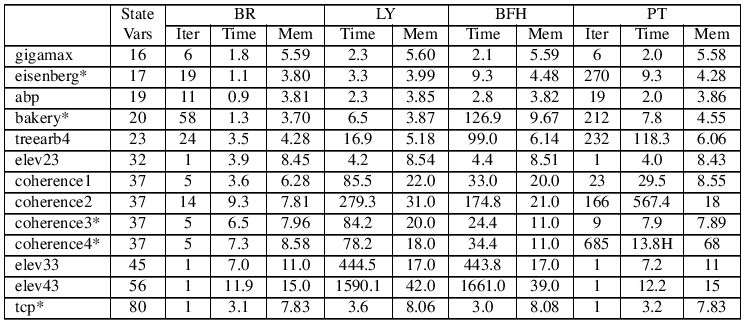
\includegraphics[width=0.9\textwidth]{figures/experimental_comparison}
    \caption{Experimental comparison of the various algorithms.}
    \label{fig:experimental-comparison}
  \end{figure}
\end{frame}

\begin{frame}
  \frametitle{Experimental comparisons}
  \begin{itemize}
  \item BR has a better time and memory usage (in almost all cases).
  \item PT does surprisingly well compared to LY and BFH
  \end{itemize}
\end{frame}

\begin{frame}[fragile]
  \frametitle{PT Optimisation}
  \begin{figure}[t]
    \centering
    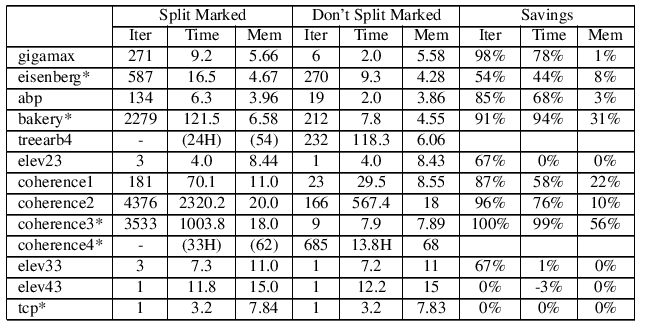
\includegraphics[width=0.9\textwidth]{figures/pt_table}
    \caption{The effect of not splitting marked blocks for PT.}
    \label{fig:experimental-comparison}
  \end{figure}
\end{frame}

\begin{frame}
  \frametitle{Experimental comparisons}
  ``That PT performs so well compared to BFH and LY suggests that minimisation
  algorithms tailored to verification settings should pay attention to choosing. ''
\end{frame}

\begin{frame}
  \frametitle{Conclusion}
  \begin{itemize}
  \item Bisimulation is very useful : minimisation technique for model checking,
    equivalence between transition systems, collapsing infinite-state systems.
  \item Assumption : the big problem is from the algorithm, not from the
    representation.
  \item Minimisation and backward reachability are similar in the spirit of
    testing invariant properties.
  \item Creation of three new algorithms : PT, LY and BFH.
  \end{itemize}
\end{frame}

\begin{frame}
  \frametitle{What to retain ?}
  Bisimulation and Model Checking require more resources than Model Checking
  alone.
\end{frame}

\end{document}